\begin{centering} 
  \huge Development of TRatioPlot in ROOT \\ 
  \large \textbf{Paul Gessinger} \\ 
  \large CERN Summer Student project \\ 
\end{centering} 
\vspace{1.5cm}
\normalsize

\noindent The ROOT data analysis and visualization framework is a software package which
is widely used in physics, especially in high energy physics. As the software became more
and more sophisticated, numerous improvements were made, and regularly, simplifications
for were achieved. 

Examples for this are the spectrum fitter and the stack facility.
A common visualization which has so far been lacking a direct implementation is the
ratio plot, as well as a few similar types of plots. The common element is a splitting
of the area into to sub areas, one of which contains the inputs, typically histograms,
whereas the other one displays the result of a calculation, as for example the result 
of a division of one histogram by the other.

While it was perfectly possible to create a plot like this in ROOT before, achieving 
a good looking result could be tedious, which led to a large number of people writing
automation on top of ROOT itself, that would take care of the process for them. The scope
and goal of my summer student project at CERN was to implement a class in ROOT itself,
that can take care of the most common types of calculations, and produces high quality
visuals. A key factor in the design was to ensure interactive usability of the class,
making it possible to explore calculation results more easily.

\begin{wrapfigure}{r}{0.4\textwidth}
  \centering
  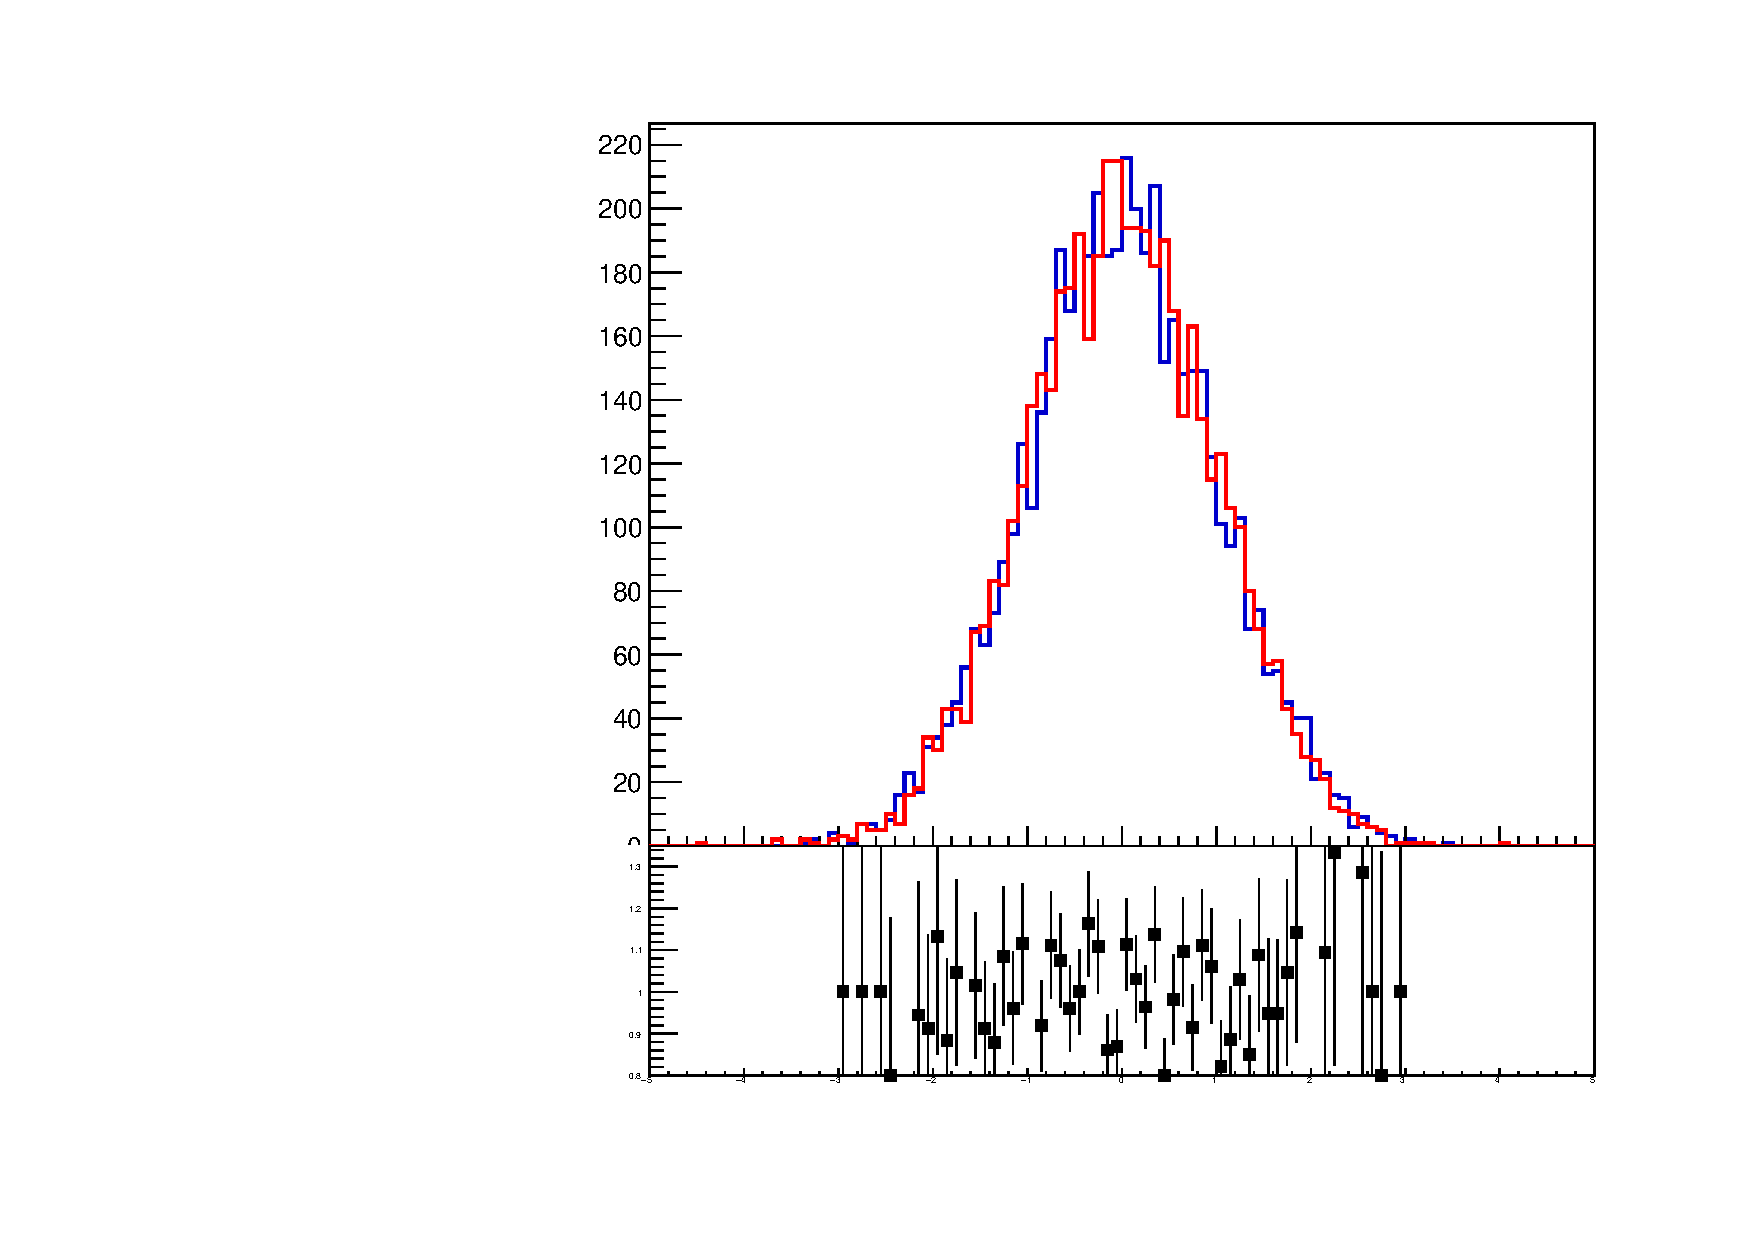
\includegraphics[width=1.0\linewidth]{assets/bad.pdf}
  \caption{Naive implementation of a ratio plot using two \texttt{TPad}s.}
  \label{fig:bad}
\end{wrapfigure}

As can be seen \autoref{fig:bad}, directly using provided facilities in ROOT yields
unsactisfactory visual results. Axis labels are sized inconsistently, as the font sizes
are derived from the size of the pad within the parent. Showing axes titles would reveal
that here sizing is also inconsistent, as are the offsets from the axis itself. A major
problem for quality is the clipping of the 0 of the upper y axis. It results from the pads meeting,
and the lower pad cutting of the overflowing the lowest label of the upper y axis.

Not visible in the static image are the issues with interactivity this implementation has. When the user
views a ROOT plot, it is possible to manipulate the visuals using the mouse. For example 
the user can zoom in by clicking and dragging on one of the axes. It is also possible to switch
the display between a linear and a logarithmic scale. Clicking and dragging on the outer frame of the 
pads allows resizing the content frame. When performing any of these actions, the pads
react completely independently, meaning changes made to one of the pads is not reflected
on the other on. This can be problematic, specifically when attempting to use the zoom
feature to explore the content, since replicating the zoomed range precisely can prove a challenge.


\clearpage

\begin{appendix}
  \section{Appendix}
  \printbibliography
\end{appendix}
